\documentclass[border=4pt]{standalone}
\usepackage{fontspec}
\usepackage{amsmath}
\usepackage{unicode-math}
\setmainfont{Latin Modern Roman}
\setmathfont{Latin Modern Math}
\usepackage{pgfplots}
\usepackage{pgfplotstable}
\pgfplotsset{compat=1.18}
\usepackage{tkz-euclide}
\usetikzlibrary{arrows.meta,calc,angles,quotes,patterns,3d,backgrounds}
\definecolor{ink}{HTML}{123428}
\definecolor{asy}{HTML}{475569}
\definecolor{mint}{HTML}{86e0bd}
\tikzset{asym/.style={asy, line width=0.9pt, dash pattern=on 5pt off 3.5pt},
         guide/.style={gray!70, line width=0.6pt, densely dotted},
         dot/.style={circle, inner sep=0pt, minimum size=5pt, draw=white, line width=0.5pt},
         odot/.style={circle, inner sep=0pt, minimum size=5.5pt, fill=white, line width=1pt},
         lab/.style={font=\footnotesize, inner sep=1.5pt, text=ink}}
\begin{document}
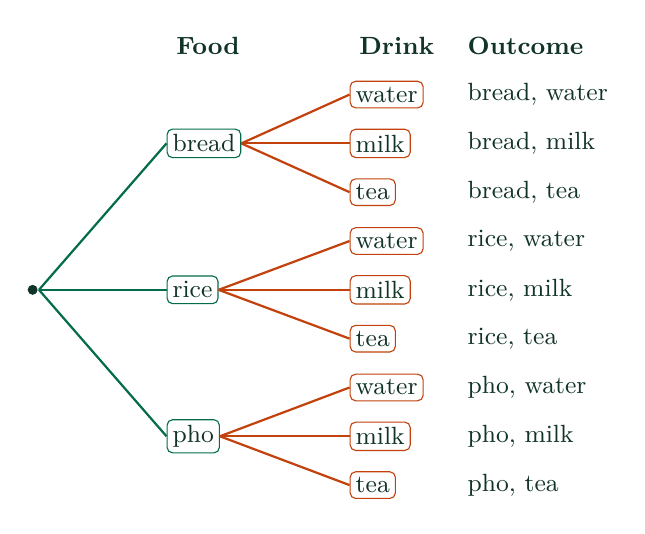
\begin{tikzpicture}
\fill[ink] (0,0) circle (1.8pt);
\node[draw={rgb,255:red,4;green,107;blue,77}, fill=white, rounded corners=2pt, inner sep=2pt, font=\small, text=ink, anchor=west] (a0) at (1.700,1.860) {bread};
\draw[color={rgb,255:red,4;green,107;blue,77}, line width=0.8pt] (0.08,0) -- (a0.west);
\node[draw={rgb,255:red,194;green,65;blue,12}, fill=white, rounded corners=2pt, inner sep=2pt, font=\small, text=ink, anchor=west] (b0) at (4.025,2.480) {water};
\draw[color={rgb,255:red,194;green,65;blue,12}, line width=0.8pt] (a0.east) -- (b0.west);
\node[anchor=west, font=\small, text=ink] at (5.400,2.480) {bread, water};
\node[draw={rgb,255:red,194;green,65;blue,12}, fill=white, rounded corners=2pt, inner sep=2pt, font=\small, text=ink, anchor=west] (b1) at (4.025,1.860) {milk};
\draw[color={rgb,255:red,194;green,65;blue,12}, line width=0.8pt] (a0.east) -- (b1.west);
\node[anchor=west, font=\small, text=ink] at (5.400,1.860) {bread, milk};
\node[draw={rgb,255:red,194;green,65;blue,12}, fill=white, rounded corners=2pt, inner sep=2pt, font=\small, text=ink, anchor=west] (b2) at (4.025,1.240) {tea};
\draw[color={rgb,255:red,194;green,65;blue,12}, line width=0.8pt] (a0.east) -- (b2.west);
\node[anchor=west, font=\small, text=ink] at (5.400,1.240) {bread, tea};
\node[draw={rgb,255:red,4;green,107;blue,77}, fill=white, rounded corners=2pt, inner sep=2pt, font=\small, text=ink, anchor=west] (a1) at (1.700,0.000) {rice};
\draw[color={rgb,255:red,4;green,107;blue,77}, line width=0.8pt] (0.08,0) -- (a1.west);
\node[draw={rgb,255:red,194;green,65;blue,12}, fill=white, rounded corners=2pt, inner sep=2pt, font=\small, text=ink, anchor=west] (b3) at (4.025,0.620) {water};
\draw[color={rgb,255:red,194;green,65;blue,12}, line width=0.8pt] (a1.east) -- (b3.west);
\node[anchor=west, font=\small, text=ink] at (5.400,0.620) {rice, water};
\node[draw={rgb,255:red,194;green,65;blue,12}, fill=white, rounded corners=2pt, inner sep=2pt, font=\small, text=ink, anchor=west] (b4) at (4.025,0.000) {milk};
\draw[color={rgb,255:red,194;green,65;blue,12}, line width=0.8pt] (a1.east) -- (b4.west);
\node[anchor=west, font=\small, text=ink] at (5.400,0.000) {rice, milk};
\node[draw={rgb,255:red,194;green,65;blue,12}, fill=white, rounded corners=2pt, inner sep=2pt, font=\small, text=ink, anchor=west] (b5) at (4.025,-0.620) {tea};
\draw[color={rgb,255:red,194;green,65;blue,12}, line width=0.8pt] (a1.east) -- (b5.west);
\node[anchor=west, font=\small, text=ink] at (5.400,-0.620) {rice, tea};
\node[draw={rgb,255:red,4;green,107;blue,77}, fill=white, rounded corners=2pt, inner sep=2pt, font=\small, text=ink, anchor=west] (a2) at (1.700,-1.860) {pho};
\draw[color={rgb,255:red,4;green,107;blue,77}, line width=0.8pt] (0.08,0) -- (a2.west);
\node[draw={rgb,255:red,194;green,65;blue,12}, fill=white, rounded corners=2pt, inner sep=2pt, font=\small, text=ink, anchor=west] (b6) at (4.025,-1.240) {water};
\draw[color={rgb,255:red,194;green,65;blue,12}, line width=0.8pt] (a2.east) -- (b6.west);
\node[anchor=west, font=\small, text=ink] at (5.400,-1.240) {pho, water};
\node[draw={rgb,255:red,194;green,65;blue,12}, fill=white, rounded corners=2pt, inner sep=2pt, font=\small, text=ink, anchor=west] (b7) at (4.025,-1.860) {milk};
\draw[color={rgb,255:red,194;green,65;blue,12}, line width=0.8pt] (a2.east) -- (b7.west);
\node[anchor=west, font=\small, text=ink] at (5.400,-1.860) {pho, milk};
\node[draw={rgb,255:red,194;green,65;blue,12}, fill=white, rounded corners=2pt, inner sep=2pt, font=\small, text=ink, anchor=west] (b8) at (4.025,-2.480) {tea};
\draw[color={rgb,255:red,194;green,65;blue,12}, line width=0.8pt] (a2.east) -- (b8.west);
\node[anchor=west, font=\small, text=ink] at (5.400,-2.480) {pho, tea};
\node[font=\small\bfseries, text=ink, anchor=west] at (1.700,3.100) {Food};
\node[font=\small\bfseries, text=ink, anchor=west] at (4.025,3.100) {Drink};
\node[font=\small\bfseries, text=ink, anchor=west] at (5.400,3.100) {Outcome};
\end{tikzpicture}
\end{document}
